\documentclass[tikz]{standalone}
\usepackage{tikz}
\usepackage{pgfplots}
\usepackage{amsmath,amssymb}
\usetikzlibrary{decorations}
\usetikzlibrary{decorations.pathreplacing, intersections, fillbetween}
\usetikzlibrary{calc,positioning}
\usetikzlibrary{plotmarks}
\usetikzlibrary{pgfplots.groupplots, pgfplots.colormaps}
\usepackage[T1]{fontenc}
\usepackage[scaled]{helvet}
\renewcommand\familydefault{\sfdefault}
\usepackage{sfmath}
\pgfplotsset{compat=newest, scale only axis, width = 11.5cm, height = 6.5cm}
\pgfplotsset{
    sciclean/.style={
        font=\footnotesize,
        axis background/.style={fill=white},
        axis on top=false,
        axis lines=left,
        axis line style={-, black},
        tick align=inside,
        major tick length=0.15cm,
        grid=none,
        enlargelimits=false,
        title style={font=\small\bfseries, yshift=0.5em},
        label style={font=\footnotesize},
        tick label style={font=\scriptsize},
    }
}

\usepackage{xparse}
\NewDocumentCommand{\onslide}{s t+ d<>}{}
\NewDocumentCommand{\only}{d<>}{}
\NewDocumentCommand{\uncover}{d<>}{}
\NewDocumentCommand{\visible}{d<>}{}
\NewDocumentCommand{\invisible}{d<>}{}

\makeatletter
\tikzset{
Sloped/.code = {
\iftikz@fullytransformed%
    \tikzset{sloped}
\else
    \pgfgettransformentries{\mya}{\myb}{\myc}{\myd}{\mys}{\myt}%
    \tikzset{sloped, transform shape, rotate = {atan2(\myb,\mya)}}%
\fi
}
}
\makeatother

\definecolor{blue}{HTML}{0072BD}
\definecolor{orange}{HTML}{D95319}
\definecolor{yellow}{HTML}{EDB120}
\definecolor{purple}{HTML}{7E2F8E}
\definecolor{green}{HTML}{77AC30}
\definecolor{light-blue}{HTML}{4DBEEE}
\definecolor{red}{HTML}{A2142F}

\begin{document}
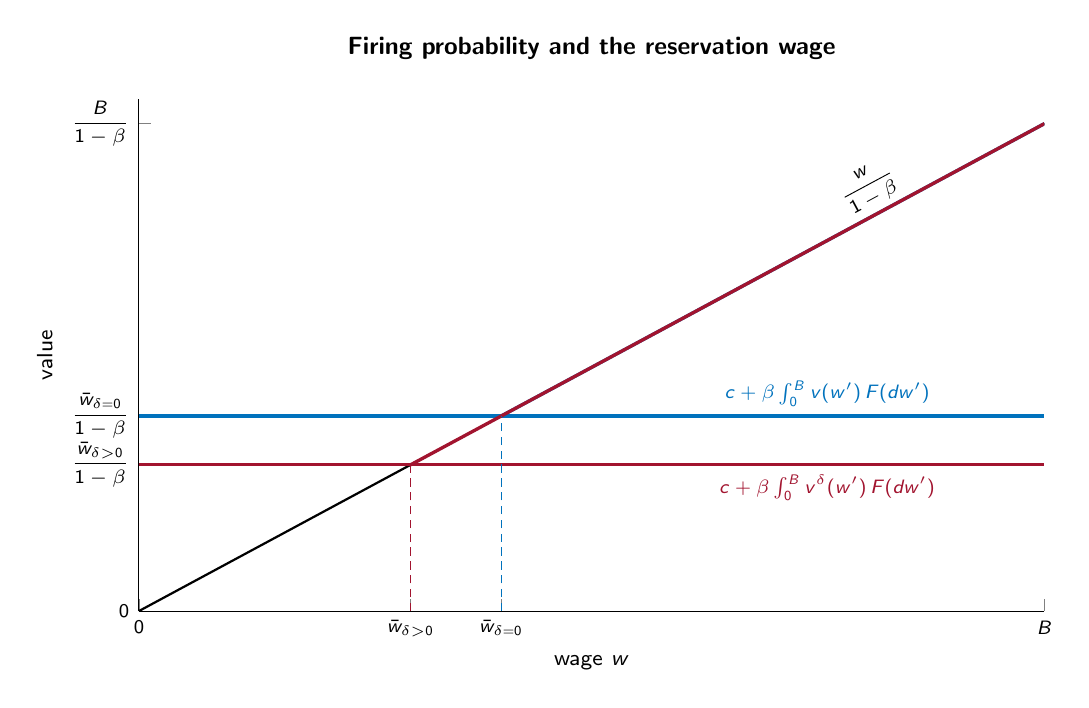
\begin{tikzpicture}

\begin{axis}[
    sciclean,
    xlabel={wage $w$},
    ylabel={value},
    xmin=0, xmax=1,
    ymin=0, ymax=10.5,
    xtick={0,0.3,0.4,1},
    xticklabels={$0$, $\bar w_{\delta>0}$, $\bar w_{\delta=0}$, $B$},
    ytick={0,3,4,10},
    yticklabels={$0$, $\dfrac{\bar w_{\delta>0}}{1-\beta}$, $\dfrac{\bar w_{\delta=0}}{1-\beta}$, $\dfrac{B}{1-\beta}$},
    title={Firing probability and the reservation wage},
]

% Normalization: 1/(1-\beta)=10 => accept value =10w.
% Baseline reject value (\delta=0): 4  => \bar w_{\delta=0}=0.4.
% With firing (\delta>0): reject value is lower: 3 => \bar w_{\delta>0}=0.3.

% Accept value line
\addplot[thick, solid, color=black, domain=0:1, samples=2]
    {10*x}
    node[pos=0.82, Sloped, above, font=\scriptsize,
         fill=white, fill opacity=0.85, text opacity=1, inner sep=1pt, yshift=1pt]
    {$\dfrac{w}{1-\beta}$};

% Reject values (constants)
\addplot[very thick, color=blue, domain=0:1, samples=2]
    {4}
    node[pos=0.76, Sloped, above, font=\scriptsize, color=blue,
         fill=white, fill opacity=0.85, text opacity=1, inner sep=1pt, yshift=2pt]
    {$c+\beta\int_0^B v(w')\,F(dw')$};

\addplot[very thick, color=red, domain=0:1, samples=2]
    {3}
    node[pos=0.76, Sloped, below, font=\scriptsize, color=red,
         fill=white, fill opacity=0.85, text opacity=1, inner sep=1pt, yshift=-2pt]
    {$c+\beta\int_0^B v^{\delta}(w')\,F(dw')$};

% Value function (baseline \delta=0): max{accept, 4}
\addplot[very thick, color=blue, domain=0:0.4, samples=2] {4};
\addplot[very thick, color=blue, domain=0.4:1, samples=2] {10*x};

% Value function (with firing \delta>0): max{accept, 3}
\addplot[very thick, color=red, domain=0:0.3, samples=2] {3};
\addplot[very thick, color=red, domain=0.3:1, samples=2] {10*x};

% Guide lines for reservation wages
\addplot[densely dashed, color=blue] coordinates {(0.4,0) (0.4,4)};
\addplot[densely dashed, color=red]  coordinates {(0.3,0) (0.3,3)};

\end{axis}
\end{tikzpicture}
\end{document}
